\section{Motivation}

% 不讲 complexity
% \subsection{Observation: Spatially Heterogeneous Computational Demands}
% During inference, Flow Matching models exhibit significant spatial heterogeneity in computational demands~\cite{jano}. Specifically, different spatial regions within a generated sample require vastly different amounts of computation, correlating tightly with their inherent visual complexity. For instance, simple, static regions (e.g., backgrounds) can reach satisfactory convergence with merely around 10 steps, whereas detail-rich, dynamically evolving subjects require the full trajectory of 50 steps. This intrinsic non-uniformity implies immense potential for content-aware selective computation. However, to truly harness this characteristic, a fundamental question remains: \emph{why does this complexity-computation correlation inherently exist?}

\begin{figure}
    \centering
    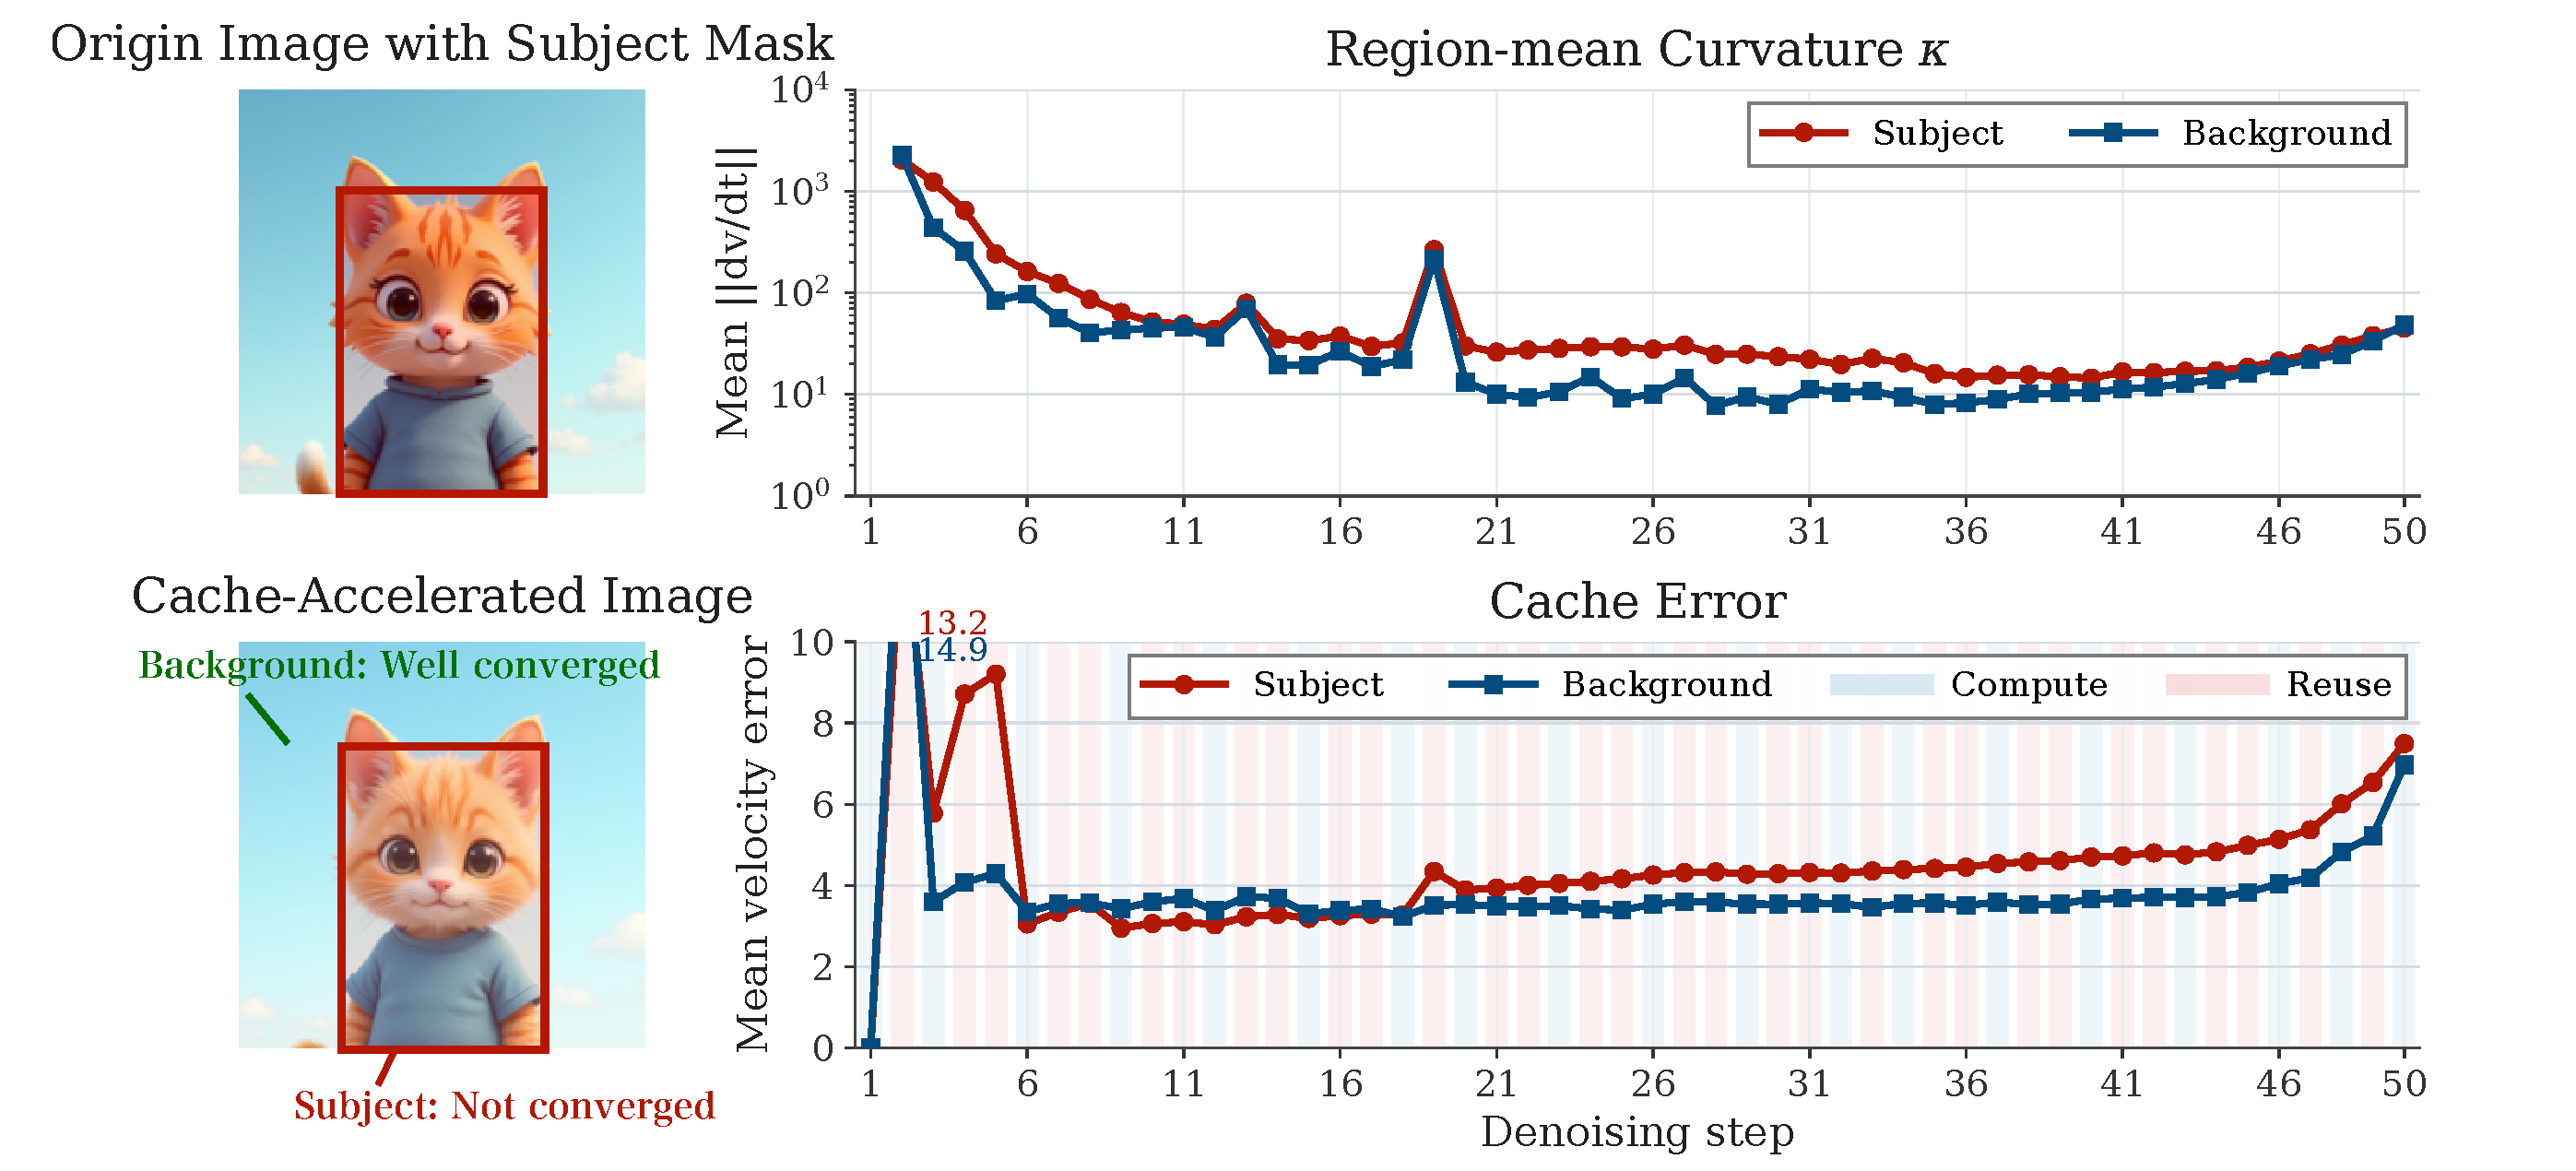
\includegraphics[width=\linewidth]{figure/motivation.pdf}
    \caption{Motivation Experiment: Subject regions exhibits higher curvature and incurs higher caching error accumulation.}
    \label{fig:motiv}
\end{figure}

\subsection{Observation: Spatially Heterogeneous Computational Demands}
During inference, Flow Matching models exhibit significant spatial heterogeneity in computational demands~\cite{jano}. Specifically, different spatial regions within a generated sample require vastly different amounts of computation to reach convergence. Usually, flat and static backgrounds converge faster than complex and dynamic subjects. This intrinsic non-uniformity implies immense potential for content-aware selective computation. However, to truly harness this characteristic, a fundamental question remains: \emph{what intrinsic property of the generation dynamics dictates these varying computational requirements?}

Fig.~\ref{fig:motiv} provides an empirical clue. Compared with the
background, the subject region shows higher trajectory curvature and accumulates
larger cache-induced velocity errors, indicating that trajectory curvature is
closely tied to region-wise cache tolerance.

\subsection{Theoretical Essence: Integration Step Size and Trajectory Curvature}
\label{sec:motiv_theory}
To understand why the cache-induced error in Fig.~\ref{fig:motiv}
varies across regions, we seek the answer from the Ordinary Differential Equation (ODE) perspective of Flow Matching. During inference, the continuous-time ODE is solved using a discrete time grid $0 = t_0 < t_1 < \cdots < t_K = 1$. Denoting the step size as $\Delta t = t_k - t_{k-1}$ (which can be uniform or non-uniform), the standard forward Euler iteration is formulated as:

\begin{equation}
    \label{wq:flow_matching_ode}
    x_{k+1} = x_k + \Delta t \cdot v_\theta(x_k, t_k).
\end{equation}
\begin{wrapfigure}{r}{0.5\columnwidth}
    % \vspace{-10pt}
    \centering
    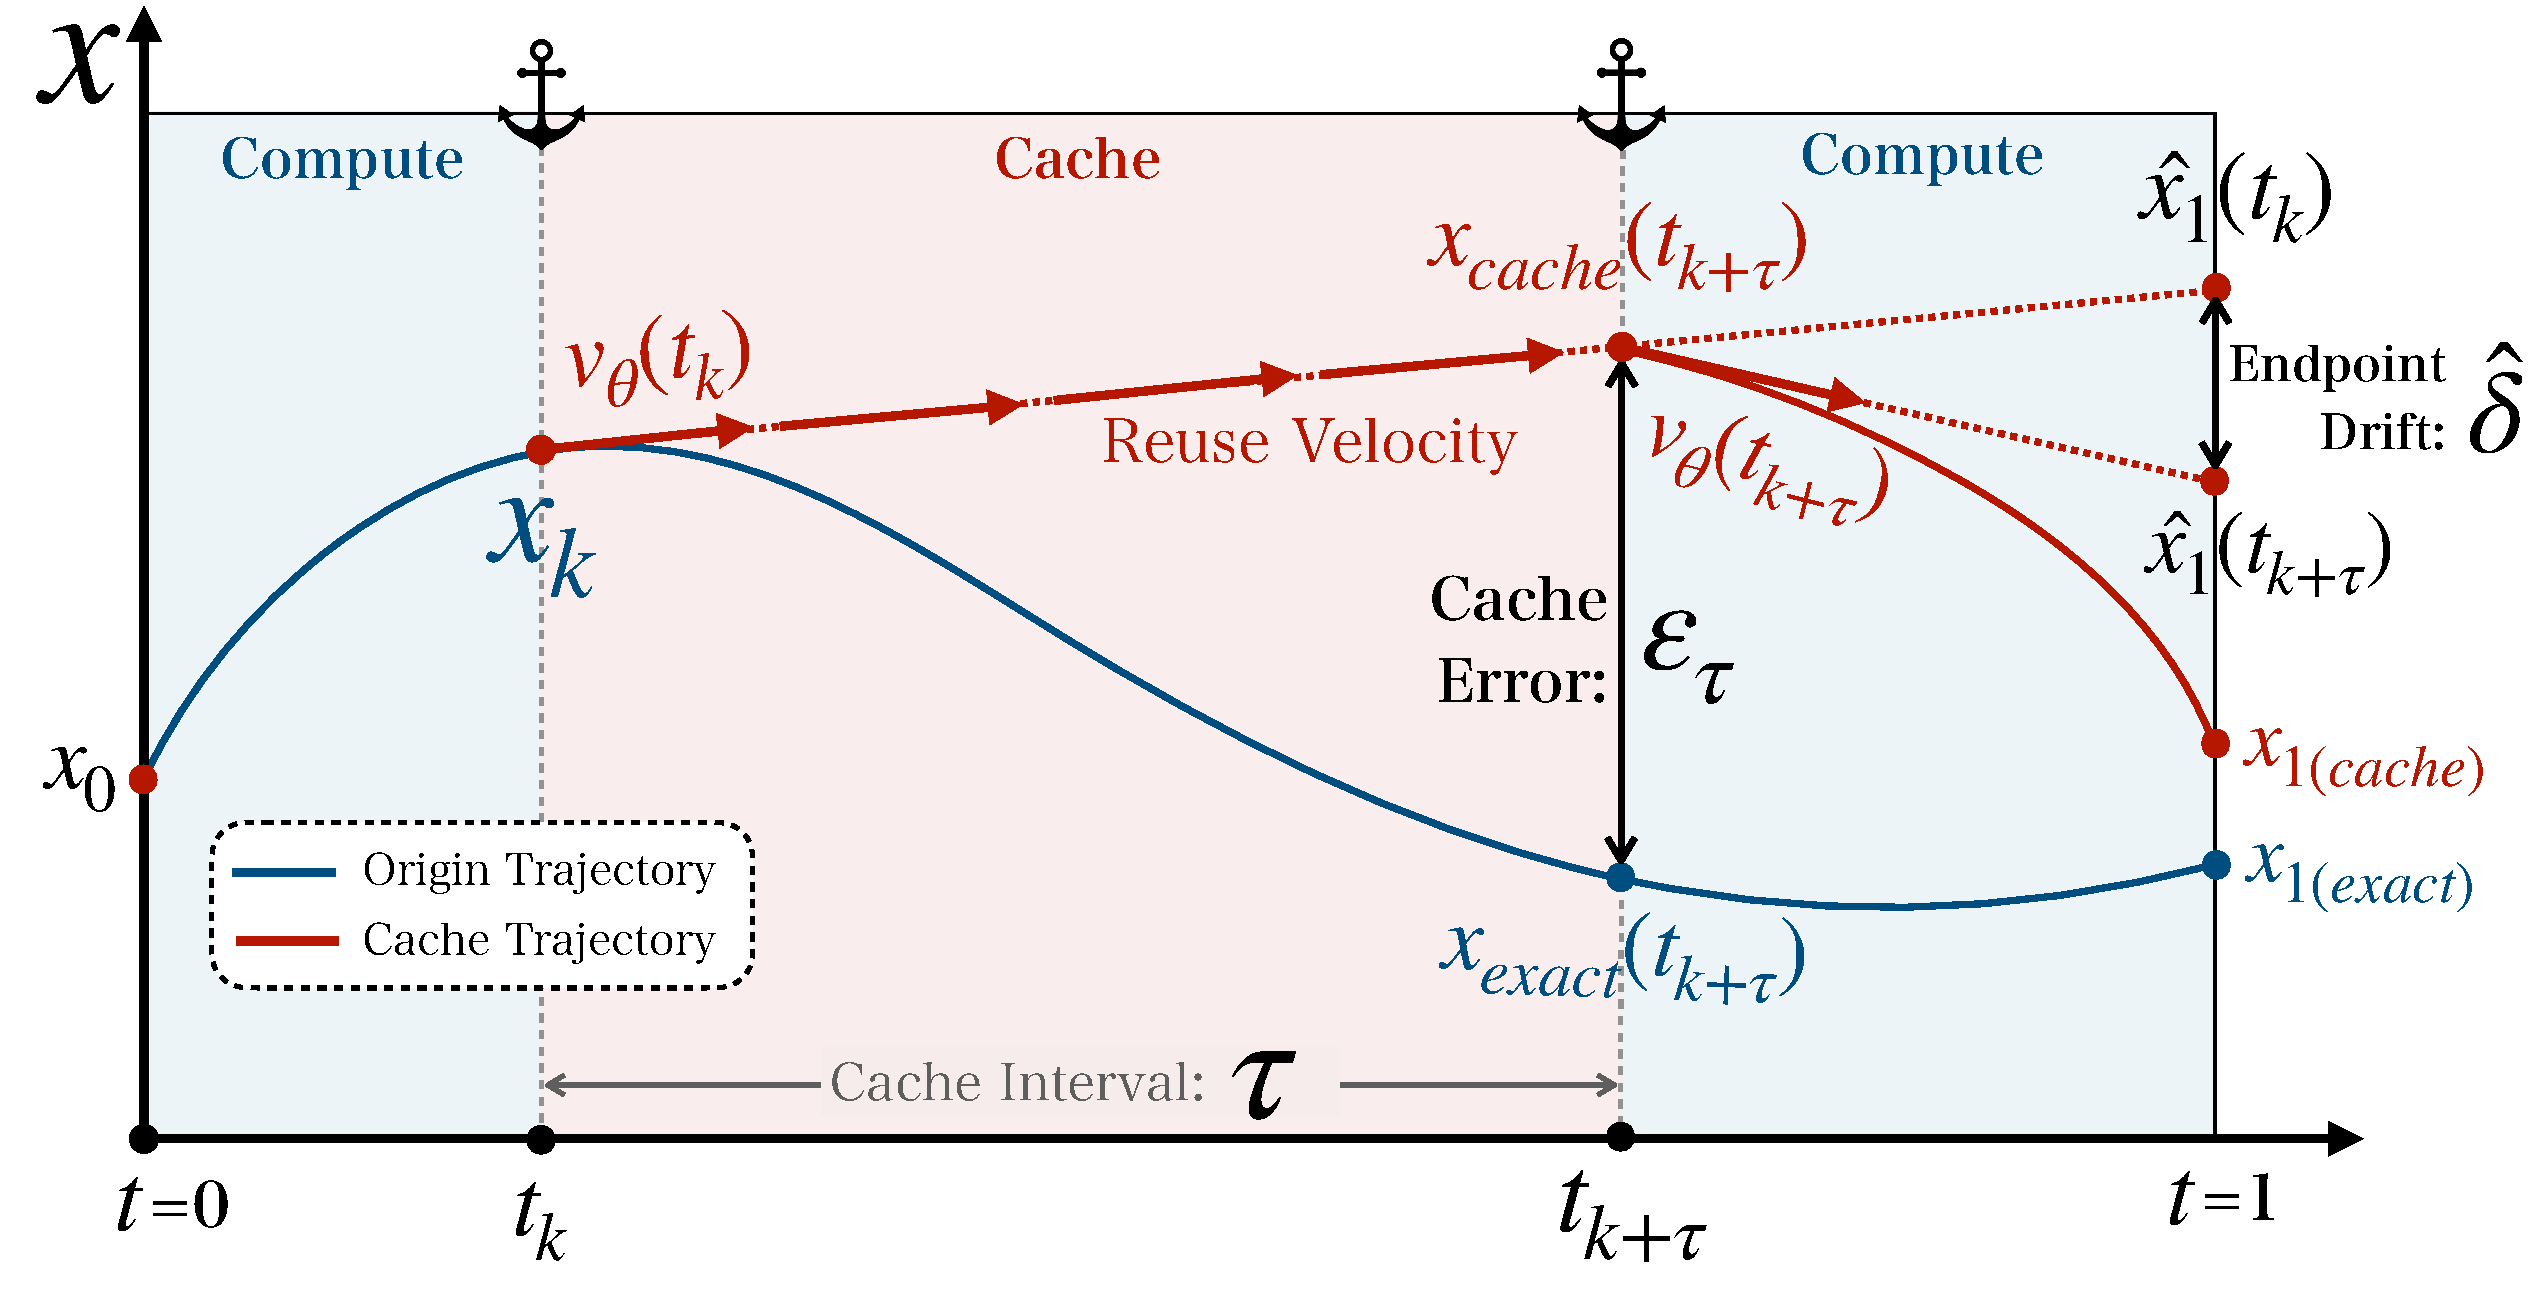
\includegraphics[width=\linewidth]{figure/method.pdf}
    \caption{Geometric interpretation of velocity reuse, cache error and endpoint drift in FM velocity field.}
    \label{fig:method}
   % \vspace{-8pt}
\end{wrapfigure}
As illustrated in Fig.~\ref{fig:method}, cache reuse can be interpreted as
holding the velocity prediction fixed over an extended interval. In other words,
reusing cached velocity features for multiple steps effectively enlarges the local
integration step size. We therefore conceptually reframe step
requirements across different regions as their
\emph{permissible integration step sizes}: fewer required updates imply that a
region can tolerate a larger effective $\Delta t$.

To achieve fast sampling, the FM training objective~\cite{rectifiedflow,meanflow}
inherently encourages the learned velocity field $v_\theta$ to be as constant as
possible along the temporal dimension, guiding the generation trajectory towards
a straight line, i.e., $dv_\theta / dt \equiv 0$. If the trajectory were perfectly
straight, a single large Euler step would solve the ODE exactly. In practice,
however, trajectories deviate from this ideal, and such deviation determines
whether enlarging effective step size is reliable.

We quantify this deviation as the \textbf{curvature} ($\kappa$) of the trajectory, mathematically captured by the material derivative of the velocity field along the flow:
\begin{equation}
    \label{eq:curvature}
    \kappa(t) = \frac{\partial v_\theta}{\partial t} + \left(\nabla_{x} v_\theta\right) \cdot v_\theta.
\end{equation}

High-curvature trajectories—driven by drastic velocity fluctuations—are highly sensitive to step size; aggressively enlarging the step introduces severe truncation errors that strictly mandate finer integration to prevent divergence. Conversely, low-curvature trajectories exhibit highly consistent velocities, where a single large step (more caching steps) is mathematically equivalent to multiple smaller ones.

\subsection{From Theory to Practice: The Practical Barriers}
While the theory dictates an optimal curvature-aware caching strategy, realizing it in practice encounters two immediate barriers. First, exact curvature is computationally forbidden. Obtaining $\kappa$ via Eq.~\ref{eq:curvature} requires computing the spatial Jacobian $\nabla_xV_\theta$ for massive sequences, introducing an overhead that completely defeats the purpose of caching. Second, the theoretical gap remains open. Even with a free oracle for $\kappa$, the exact mapping from ODE trajectory curvature to the actual feature-reuse "staleness error" is mathematically undefined. Without a closed-form error bound, any curvature-based design inevitably falls back into the trap of empirical tuning, lacking the formal guarantees needed for true optimality.